\chapter{Introduction}

\section{Motivation}
%heranführung zum thema, erklären warum das wichtig ist.
In recent years, Mixed Reality (MR) devices became more affordable \footnote{\todo}, portable \footnote{\todo} and usable in more conditions. Not only academic researchers are interested in this technology, commercial companies also found MR devices helpful to explore new possibilities to use it profitable. With this development, learning and training in MR became possible for many cases, too. EON \footnote{\hyperlink{https://www.eonreality.com/}{https://www.eonreality.com/} accessed: 14.12.2018} for example calls themself "the world leader in Virtual Reality based knowledge transfer for industry, education, and edutainment". They develop MR programs for several platforms, eg. with the aim to guide workers, reducing mistakes and thus reducing costs. These programs address a lot of usecases in the field of education, energy, health \& medical, manufacturing \& industrial, defence \& security and aerospace. Tasks include eg. ground crew training for a Boeing 777, augmented reality (AR) assembly training, exploring or anatomy simulation to mention only a few, compare \ref{fig:eonreality}.
\begin{figure}
	\centering
	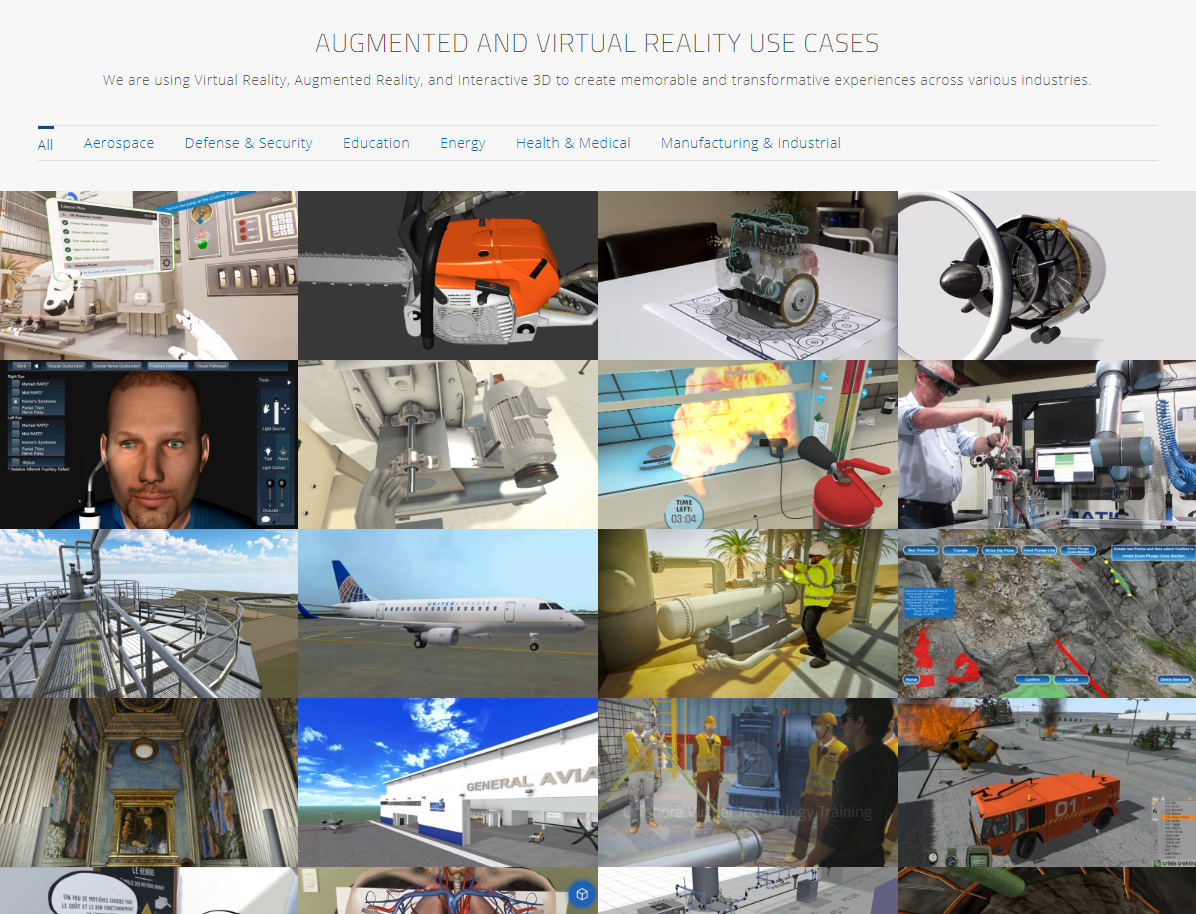
\includegraphics[width=1.0\textwidth]{img/eonreality.PNG}
	\caption{Usecases by EONReality on their AVR plattform.  \hyperlink{https://www.eonreality.com/use-cases/}{https://www.eonreality.com/use-cases/} (accessed 30.07.2019)}
	\label{fig:eonreality}
\end{figure}
Mircosoft also stepps into this topic with partners, developing tools for apprentice, maintenance, or remote training. Eg. The Smart Glass experience Lab\footnote{\hyperlink{https://www.fit.fraunhofer.de/de/fb/cscw/smart-glasses-experience-lab.html}{https://www.fit.fraunhofer.de/de/fb/cscw/smart-glasses-experience-lab.html}} of the Fraunhofer Institute use the hololens for remote maintenance.
\begin{figure}
	\centering
	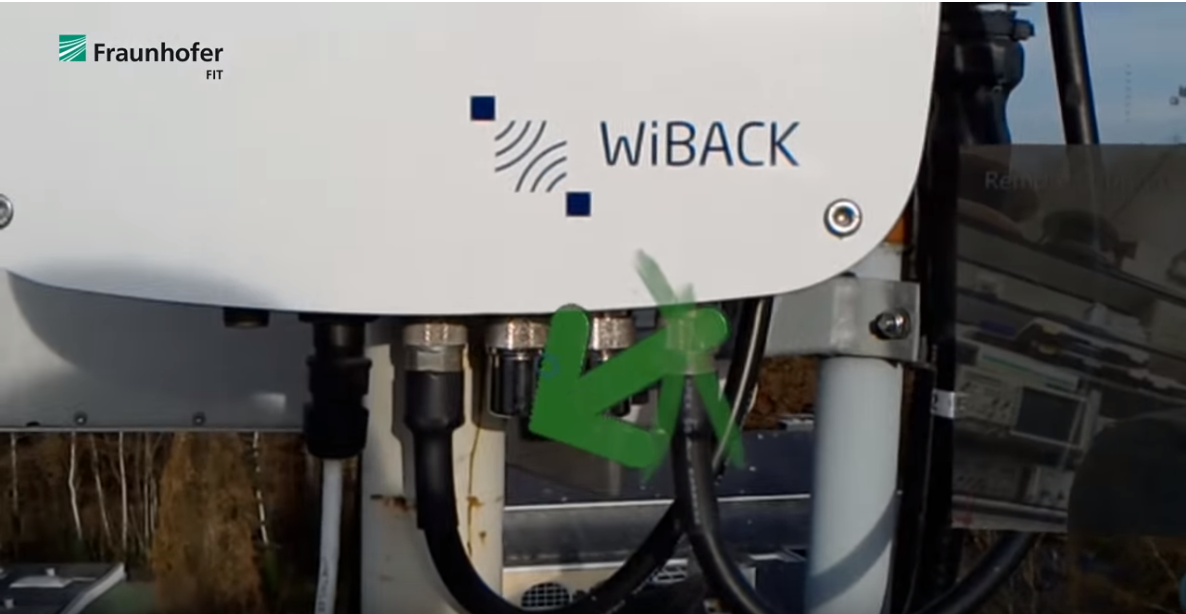
\includegraphics[width=1.0\textwidth]{img/fraunhofer.PNG}
	\caption{Remote maintenance with Hololens by Smart Glass Experience Lab. The on site worker wears a Hololens, while the remote trainer draws green hints to resolve a miswiring, taken from \hyperlink{https://www.youtube.com/watch?v=1QFMPo5k6p0}{https://www.youtube.com/watch?v=1QFMPo5k6p0}, accessed (30.07.2019)}
	\label{fig:eonreality}
\end{figure}\\
For developing MR learning and training environments, research put much afford in developing how-to's and guidelines to ensure proper systems. However - as we will see in Chapter 4 - there is a research gap about the perspective in these systems. For example, a student wants to learn a speacial task from a teacher. In the real world, the teacher stands in front of the student preforming the task and the student tries to mimic it. This perspective is called exocentric or 3rd person. In contrast, in MR we have the possibility to change this perspective what we cannot do in the real world. We can "step into" the teachers virtual body and see the instruction from the 1st person view of the teacher, also called egocentric view. Changing the perspective could have influence on the learning. This rises the following question: Does the perspective has influence on learning in MR environments? Furthermore, to develop guidelines for MR learning environments, it would be helpful to know if the there are conditions where either of this perspectives is more suitable than the other. Since learning and training in MR is a vast area, the topic is narrowed down to the subset of motor learning. 
This seminar thesis is the first out of three parts, followed by a Masters Project and a Masters thesis. The overall aim of this work is to answer to following research question:
\begin{itemize}
	\item[RQ1] Does the perspective on a virtual avatar has influence on learning in MR environments.
	\item[RQ1.1] Are there conditions, under which one perspective works better than the other.
\end{itemize}
The outcome in this work is a study design that will be able to address the research questions. In the Masters project the proposed study setting will be implemented, to be able to conduct the study and collecting the data necessary to answer the question. The Masters thesis itself will take the generated data to answer the research question.


\section{Outline}
For a proper study design many aspects must be taken into consideration. The main aspects this thesis will discuss are defined in the following, while further aspects like algorithms are discussed in the masters project.
\begin{itemize}
	\item[A1] independent variables%t
	\item[A2] dependent variables%p
	\item[A3] movement classification%t
	\item[A4] open vs. closed skills%t
	\item[A5] task%p
	\item[A6] perspective%t
	\item[A7] MR vs. VR%t
	\item[A8] MR technology%p
	\item[A9] tracking technology%p
	\item[A10] synchronous vs. asynchronous instructions%t
	\item[A11] behaviour of instructions%p
	\item[A12] measures%p
	\item[A13] considered body parts%p
	\item[A14] degree of realism of the avatar%t
	\item[A15] feedback%t
\end{itemize}
Each of these aspects must be chosen wisely. In order to do so this seminar thesis will systematically go through every one of them. Chapter 3 provides insight to these aspects from a theoretical view. In addition, this chapter provides general knowledge about the domain. In contrast, chapter 4 takes the work of other researchers into consideration. Here, the aspects are analysed from a more practical view and it is investigated how these researchers decided about the aspects and why. Whenever a decision is made to be used in the proposed study design, a symbol on the side of the text can be found\markA. After all aspects are clear and reasoned, a study design is proposed in chapter 5. In the end, an outlook on further work on the Masters thesis is given and highlighted what aspects are still to decide of.

\todo graphical representation

%first the theoretical background will be taken into consideration. It is mandatory to know how humans learn, classify, quantify and measure movements. In addition, recent MR hardware and tracking technology is investigated, a classification of perspectives is given and also a insight on MR itself. In this chapter we also set the res
%This seminar thesis will have a look at the grounding principles to define a system that lead to the guidelines in question. Therefore we first step into the theoretical background in the next chapter. We will investigate how people achieve motor skills, how to quantify and measure movements, what hardware techniques are suitable, perspectives and mixed reality. In the following chapter we analyse how other researchers used the theory to gain insights in Motor learing in VR. In the end we propose a study setting to that can be used to investigate on this topic.
%After this introduction, the scope of this thesis is given, where it is explained to what extend motor learning, MR, perspectives and other factors are considered. The following related work part will give an overview about other MR learning systems and also work about perspectives on avatars. From this work the measures, dependent and independent variables and tasks are derived. Taking the related work into consideration a study design is proposed in outlook section.